\chapter{Design And Architecture\label{chap:design}}

This chapter describes the design of the system. This includes both the underlying decisions as well as the user interface design. The chapter also presents a more detailed view of the system's architecture.

\section{System Design}

The system has to work in two major steps. The first step is to take a semi-structured natural language script and analyse it. This means that the system must analyse each dialogue line and infer some emotional values from it. Using those emotional values and the length of the dialogue line, the system must find best matching animation clips from the motion capture database. The result of this step is a file that specifies which characters say which lines of dialogue and which animations to use while they are talking.

After this step is completed, the file must be interpreted into a final scene. The generator must be able to read the file, import required models and animations and generate the final scene. As every animation software and game engine is a little different, each of them would need a custom generator. Those would be very similar in principle, but differ slightly because of the implementation of a given software. For my project I have created the generator module for Blender.


\section{Emotions}

For my project I have decided to only use the following emotions: joy, fear, anger and sadness. Traditionally, surprise and disgust are also part of the six basic emotions model by Paul Ekman and Wallace V. Friesen. However, IBM Watson Tone Analyzer, that I am using for sentiment analysis, is unable to detect surprise in the text (more on that in section ~\ref{sec:emoanal}) and the disgust emotion is not well represented within the EBMD. Therefore, I had to abstain from using these emotions in this project. 

The emotions are expressed as decimal fractions between 0.0 and 1.1 - this identifies whether a given emotion is present in a specific motion clip or text and how intense that emotion is. It also allows to create a mixture of emotions in order to represent more complex emotions. The EBMD describes the animations in terms of their emotion category, but provides no value (the EMDB does not differentiate between an angry gesture and a \textit{very} angry gesture). Therefore each animation clip has to be manually reviewed in order to assess its emotional properties.

\section{Architecture}

The architecture of the system is essentially a pipeline. The modules process resources and pass them onto the next module while being unaware of each other. This allows for a lot of flexibility and helps achieve some of the requirements. The emotion analysis API can be replaced with a different one, the user can use a custom motion capture database, and a different generator can be created if the user wishes to use software other than blender.


There are three main modules:
\begin{itemize}
\item Text Analysis
\item Animation Clip Matcher
\item Animation Generator
\end{itemize}

The Text Analysis module parses the text and analyses emotion using some API (IBM Watson). It takes a script as an input and passes the parsed and analysed text to the Animation Clip Matcher.

The Animation Clip Matcher uses the motion capture database to find the best animation clips to accompany the speech. The Animation Clip Matcher must take into account the emotion analysis of the text and find animations with similar emotional score. Another important constraint is the time of the animation. The animated clips have different lengths and a chosen clip must not be significantly longer than the spoken/read text. The Matcher outputs a JSON file which specifies all dialogue lines; it states which characters perform which emotional gesture actions and where the animation file is located.

The Animation Generator reads the JSON file and imports all needed animations. The user is now able to assign a character model to each character and run the generator. The generator will assemble the animations in correct order, focus the camera on a currently speaking character and add subtitles. The output is an animated scene that can be either manually edited, exported to a file or rendered.

The full diagram of the system can be seen in figure ~\ref{fig:architecture}.

\begin{figure}[!ht]
\centerline{\fbox{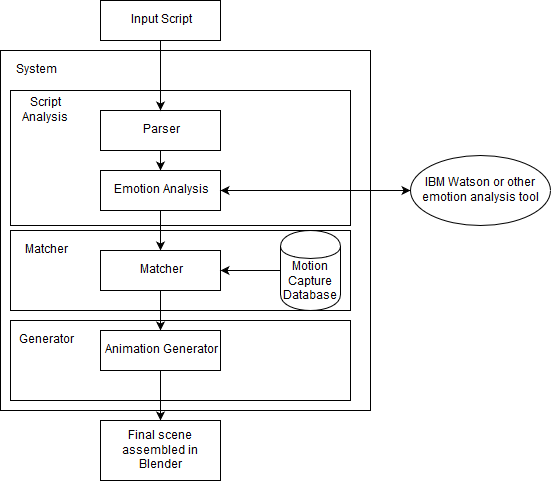
\includegraphics[width = 30em]{img/architecture.png}}}
\caption{The pipeline architecture of the system}\label{fig:architecture}
\end{figure}

\section{Character Armature and Model}

As the system is designed to be used in games, one of the main requirements for the system is to handle various character models. Because, in a game, each character is represented by a different model, this is a necessity. The model itself is relatively irrelevant - it must however support the same or similar enough armature\footnote{Armature - a skeleton of a character model.} to the armature the system was designed around. The armature used in this project is shown in detail in figure ~\ref{fig:armature}. For an armature to be supported, the bones must have corresponding names. Any extra bones or bones with unmatching names will be left not animated.

\begin{figure}[!ht]
\centerline{\fbox{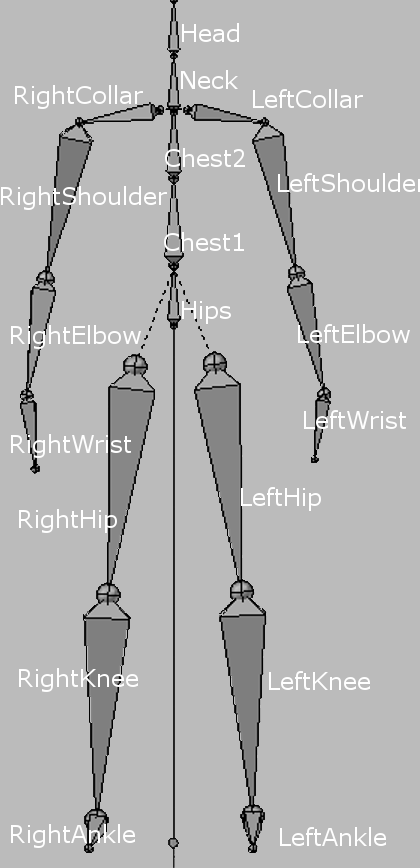
\includegraphics[width = 20em]{img/armature.png}}}
\caption{The armature supported by the system}\label{fig:armature}
\end{figure}


\section{EBMD Importer and Showcase Generator}
The following are small tools created to help automate / bootstrap the process of acquisition and categorization of the animations.


\subsection{EDMB Importer}
The EBMD importer's purpose is to help prepare the animations obtained from EBMD to work with the system. The EBMD animations have a few issues making them incompatible with the system - The armatures are a little different with unmatching bone names, many animations were recorded while actors were sitting down \footnote{Leg animation is irrelevant for this system.} and are saved in BVH files \footnote{BVH files are suitable for motion capture, but can be more problematic for generic animation than FBX.}.

\medskip
\noindent To import an animation, the importer must follow through the following steps:
\begin{enumerate}
\item Download animation from link to file (receive http link as input) and import the animation from the downloaded BVH file.
\item Remove animation data from the legs.
\item Rename the bones that the animation data applies to so that they match those of the target armature.
\item Import the target armature.
\item Apply the action (animation data) imported from EBMD to the target architecture.
\item Export the animation data to FBX file format.
\end{enumerate}

The EMDB importer helps automate the process of acquiring animations by enabling downloading and processing a huge bulk of animations, saving them in folders that correspond to their emotion category and showing their length in frames in the filename.

\subsection{Showcase Generator \label{sec:showcasegenerator}}
The purpose of the showcase generator is to help categorize and store the animations in the database (section ~\ref{sec:dbdesign}). The showcase generator outputs instructions for the animation generator (section \ref{sec:generatordesign}) which allow the animation generator to create an animation which shows all the animations in a given directory, one after another. Since the animations have to be analyzed manually (in order to assess their emotional value), a clip showing all animations allows for a quick and easy analysis.


\section{Input}

The input of the system is a file that represents a dialogue. Each character that participates in the scene must be clearly stated. Each dialogue line must have a character clearly associated with it. Character names are specified after five tabs. Dialogue lines are specified after three tabs. Each file must end with ``ENDSCRIPT'' with no indentation.

I used this format as this format is often used to represent movie scripts. One can find hundreds of scripts saved in this or similar format in The Internet Movie Script Database (\url{www.imsdb.com}). An example input can be seen in figure ~\ref{fig:inputscript}.


\begin{figure}[H]
\centerline{\fbox{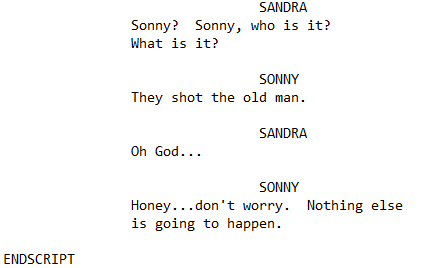
\includegraphics[width = 30em]{img/script.png}}}
\caption{An example of system's input}\label{fig:inputscript}
\end{figure}


\section{Emotion Analysis} 
\label{sec:emoanal}
As aforementioned, there are many ways to perform emotion analysis of the text. I have chosen to use IBM Watson Tone analyser for this task as it offers a state-of-the-art service accessible for prototyping.

The module takes each dialogue line and sends to IBM Watson Tone Analyzer for analysis. Watson's REST API is used to accomplish that. The API returns all the emotion values between 0.0 and 1.0 found in the text. Each dialogue line now has emotional values assigned to it.

\section{Database}
\label{sec:dbdesign}

The motion capture database consists of two main parts: the files that contain the animated clips and a database that holds the meta-data about the animations and character models.

The animation data is stored in FBX files - one animated action per file. The folder structure can be customized - for the purposes of this project the animations are stored in a way that describes the emotions they convey \footnote{For example: animations > anger > subtle > disbelief1.fbx}. The folder structure is irrelevant as long as it stays consistent with the entries in the SQLite database. 

The database is implemented using SQLite. It is the perfect tool for this task as the database needs to be simple, relatively small and easily searchable. The animation meta-data is held in a table presented in figure ~\ref{fig:db}. The emotional values of each animated clip need to be manually adjusted. When all values are set to zero, it means that the clip carries no emotional impact (the clip is neutral). An example of a few database records can be seen in figure ~\ref{fig:db}.

\begin{figure}[H]
\centerline{\fbox{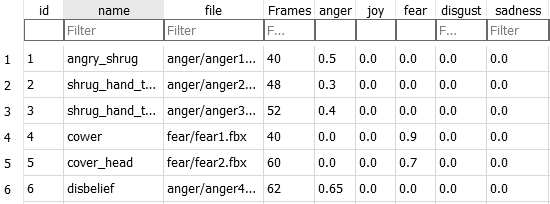
\includegraphics[width = 30em]{img/db.png}}}
\caption{Database of animation clips}\label{fig:db}
\end{figure}

The other purpose of the database is to store the information about the character models. The important information about a model is its name, file location, camera offset and rotation. Because models may be of different shapes and sizes, camera positioning during dialogue will not be the same for every model. The database allows to specify a desirable camera position relative to the character that will allow to fully capture the character at a good angle. Example of a few model database records can be seen in figure ~\ref{fig:dbmodel}.

\begin{figure}[H]
\centerline{\fbox{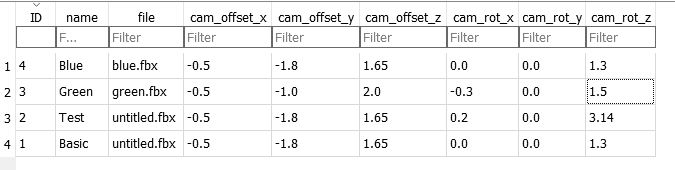
\includegraphics[width = 30em]{img/dbmodel.png}}}
\caption{Database of character models}\label{fig:dbmodel}
\end{figure}


\section{Matcher}

The matcher module depends on the emotion analysis and database modules. It takes the emotion data and searches the database for a suitable animated clip. The matcher's input is a dictionary where the keys are emotions (anger, fear, etc.) and values are 0.0 to 1.0 decimals.

\subsection{Score matching}
\label{sec:scorematching}
Firstly, the matcher will decide whether the text carries enough emotions. If no emotion surpasses the constant relevancy threshold (in this project the threshold is set to 0.2) the animation is deemed as neutral. If there is only one emotion that exceeds the threshold, the module will look for an animation matching that emotional value. If more than one emotion exceeds the threshold, only the two most important (highest value) emotions will be considered. That is because certain emotions often go in pairs (such as anger and sadness), but combinations of more than two emotions are rare, confusing and hard to represent with an animation. The module searches the database for animations that may be fitting and compares the text emotional values with the animation's emotional values. The pseudocode behind these calculations can be found in figure ~\ref{fig:matcher}.

\subsection{Length Matching}
The matcher must account for the fact that even the most emotionally fitting animations may not be the most suitable. It is very important to take into account the length of the speech - the length of the gestures performed in an animation must match the length of a character's dialogue line. Otherwise, there will be situations where a short animation is chosen for a few sentences worth of dialogue, or a very long animation is chosen for just a few spoken words.

To account for this, constant frames per second (to define animation length in real world terms) and words per second (to calculate the length of a dialogue line in seconds) must be defined. The matcher uses those to calculate the ratio between an animated clip length and speech length. This ratio is used to adjust the score calculated using emotional values (section ~\ref{sec:scorematching}). How the two matching operations work together can be seen in the pseudocode in figure ~\ref{fig:matcher}.

\begin{figure}[!ht]
\centerline{\fbox{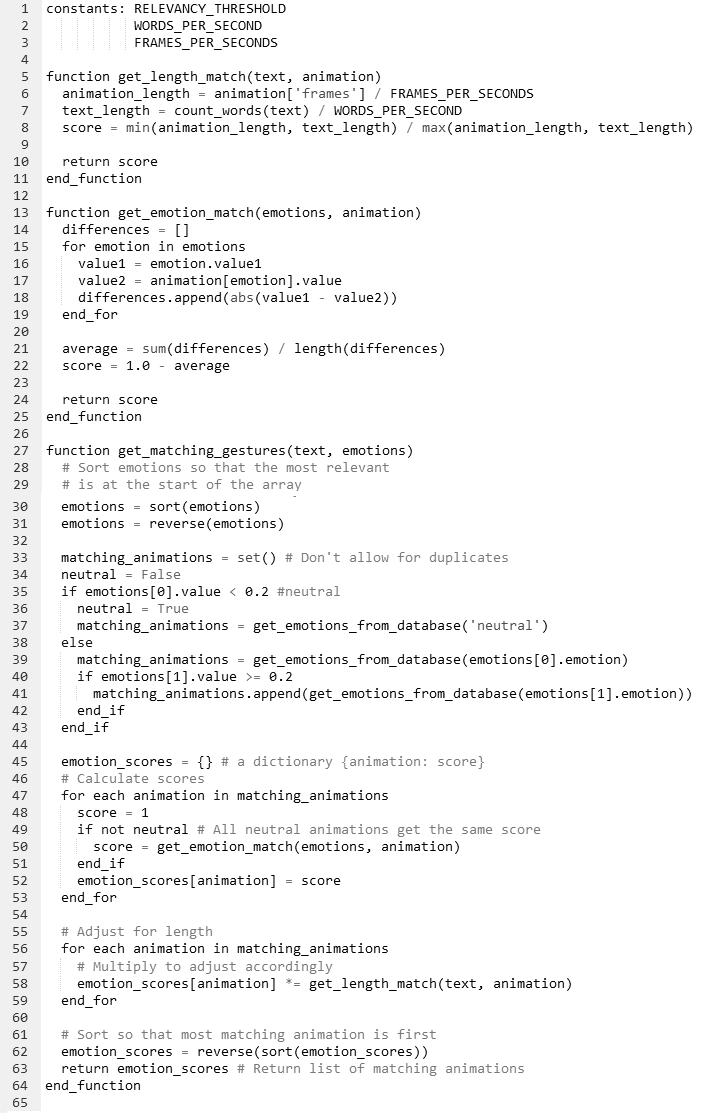
\includegraphics[width = 30em]{img/matcher.png}}}
\caption{Pseudocode explaining how the matcher calculates the scores}\label{fig:matcher}
\end{figure}

Additionally, the matcher will ensure that the animation is not too monotonous. The matcher will not choose the same animation twice in one dialogue - it will prioritize a similarly matching animation that has not yet been used. The animations will be reused if no other matching animations are available.


\section{Animation Generator (Importer)}
\label{sec:generatordesign}

As aforementioned, in this project I have used Blender to support the animation generator module. The generator is a Blender add-on.  It can either be used as a script, or be installed as an add-on in order to be fully and permanently available within Blender.

The generator first reads the JSON file prepared by previous modules and pre-loads required animation clips from files. The user needs to assign a 3D character model to each character participating in the scene. The required 3D character models are animated and the camera is positioned accordingly to the model's meta-data. The animated characters are positioned to directly face each other (the program currently supports only up to two characters in one scene). Each animated action is assigned to a corresponding character model and then pushed on a separate NLA strip (figure ~\ref{fig:nla}). The program keeps track of how many frames are being used so that the newly added actions begin just when the previous actions end.

To setup some basic background and feel, a floor (plane) is added beneath the characters and two directional lights cast light down from above the characters.

The camera is added to the scene and positioned using the meta-data retrieved from the database. At the start of each character's actions the camera is positioned and rotated to focus on the character that is currently speaking.

Subtitles are added as Video Editor Sequence Strips spanning between frames that correspond to the animation (figure ~\ref{fig:substrips}).

\begin{figure}[H]
\centerline{\fbox{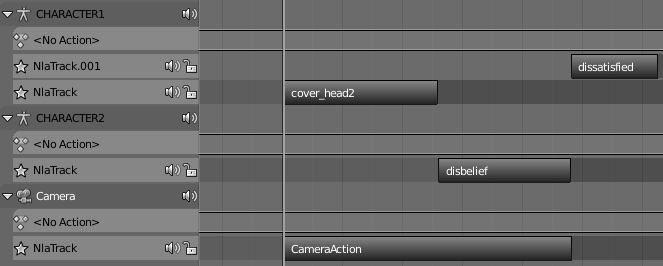
\includegraphics[width = 30em]{img/nla.png}}}
\caption{NLA strips of the final animation}\label{fig:nla}
\end{figure}
\begin{figure}[H]
\centerline{\fbox{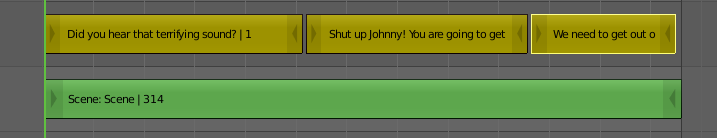
\includegraphics[width = 30em]{img/substrips.png}}}
\caption{Video strips featuring subtitles}\label{fig:substrips}
\end{figure}

The final animation can be edited and adjusted in Blender (figure ~\ref{fig:finalblend}), rendered (figure ~\ref{fig:finalrend}) or exported to file.


\begin{figure}[H]
\centerline{\fbox{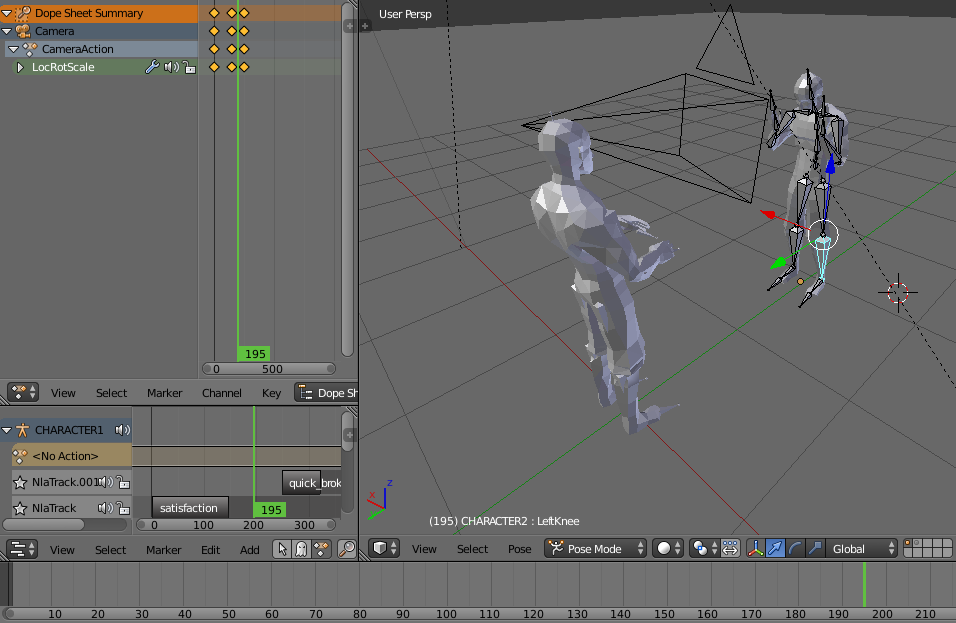
\includegraphics[width = 30em]{img/finalblend.png}}}
\caption{Editing the final animation in Blender}\label{fig:finalblend}
\end{figure}
\begin{figure}[H]
\centerline{\fbox{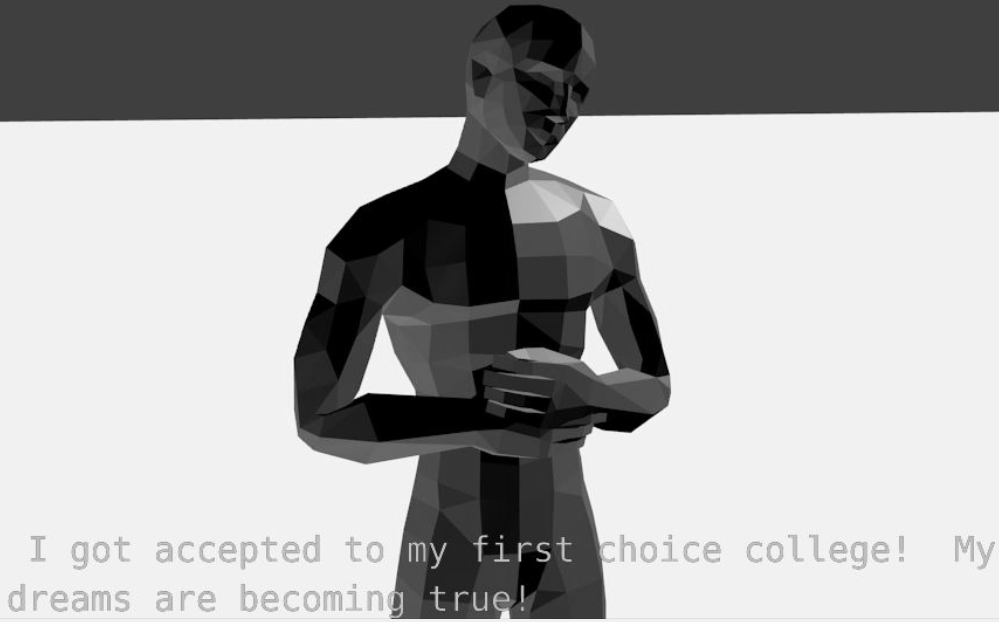
\includegraphics[width = 30em]{img/finalrend.png}}}
\caption{Rendered final animation}\label{fig:finalrend}
\end{figure}

\section{User Interface}

The Animation Generator module is the only module that features a Graphical UI. The module is embedded into Blender and uses extends Blender's interface. 

The UI is minimalistic and simple to use. Upon installation and activation, a new tab is added to the menu on the left-hand side. Figure ~\ref {fig:ui_main}. Rectangle 1 represents the left hand side menu. Number 2 shows the tabs, where the bottommost one belongs to the extension. Number 3 shows the actual UI of the extension.

\begin{figure}[H]
\centerline{\fbox{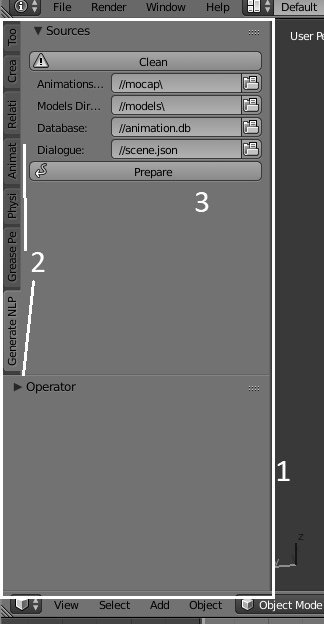
\includegraphics[width = 18em]{img/ui_main.png}}}
\caption{The addon UI}\label{fig:ui_main}
\end{figure}

From there the user is able to either clear the scene (might be useful especially if something unexpected happens or the work of the extension have been interrupted and requires a restart) or prepare the scene. To prepare the scene the user must first initialize the four variables. The user needs to point the program to where the animations and models are stored as well as to where the database file and the scene file can be found (JSON file generated by previous modules).

Upon pressing `Prepare' the program will prepare for scene generation. Required animations will be imported and the scene file will be parsed. There is one more step left to finalize the animation. When preparation is finished, a new menu will pop up below the currently existing one. The menu can be seen in figure ~\ref{fig:ui_finalize}. In the menu the user is required to assign a character model to each character existing in the scene. Upon pressing `Assemble' the full scene will be generated complete with lighting, camera movement and subtitles.

\begin{figure}[H]
\centerline{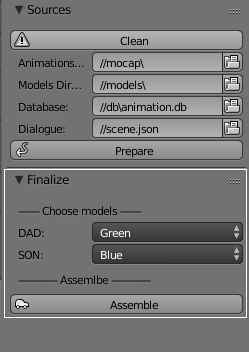
\includegraphics[width = 18em]{img/ui_finalize.png}}
\caption{The finalization step (new menu highlighted by white rectangle)}\label{fig:ui_finalize}
\end{figure}

They key aspect of the interface is its simplicity as it allows users to generate relatively complicated animation sequences by essentially using two buttons, with no knowledge about animation and little Blender expertise required. The UI also provides flexibility as the user can decide which character models to use.





